\documentclass[a4paper,10pt]{article}
\usepackage[utf8x]{inputenc}
\usepackage[spanish]{babel}
\usepackage[utf8x]{inputenc}
\usepackage{verbatim}
\usepackage{hyperref}
\usepackage[pdftex]{graphicx}
\usepackage{wrapfig}

\usepackage{anysize}
\marginsize{1.5cm}{1.5cm}{1cm}{1cm}

%\usepackage{sectsty}
%\sectionfont{\Large}

\pdfinfo{%
  /Title    (Trabajo Práctico Especial)
  /Author   ()
  /Creator  ()
  /Producer ()
  /Subject  ()
  /Keywords ()
}

\begin{document}

\begin{titlepage}
\begin{center}
 \huge \underline{\textbf{Trabajo Práctico Especial}}\\[0.05cm]
 \normalsize \textbf{Protocolos de Comunicación}\\[0.25cm]
 \normalsize \textbf{Revisión correspondiente a la entrega: }\\[1cm]

\large
\begin{tabular}{c @{ - } l}
 Andrés Mata Suarez & 50143 \\
 Jimena Pose & 49015 \\
 Pablo Ballesty & 49359 \\
\end{tabular}\\[19.4cm]
 2011 - Segundo cuatrimestre
\end{center}

\end{titlepage}

\setcounter{tocdepth}{2}
\tableofcontents


\newpage

\section{Descripción detallada del protocolo desarrollado}

\subsection{RFC}
A continuación se presenta el RFC del protocolo \textit{configurotocol 1.0}, diseñado para manejar la configuración
del servidor proxy.

\verbatiminput{configurotocol2.txt}

\subsection{Consideraciones}
Se decidió basar el formato del protocolo en JSON, ya que este es fácil de leer y escribir para los usuarios y es
fácil de parsear y generar para las máquinas. Por otro lado, facilita mucho el parseo del archivo de configuración,
ya que el mismo también se guarda en formato JSON. Por lo tanto, al momento de configurar el proxy, la generación 
e interpretación de comandos no debería ser ningún problema, tanto para un usuario como para una máquina.\\
Es importante destacar que todos los cambios exitosos de configuración son persistidos. Por lo que ante cualquier
inconveniente, en caso de que el proxy deba reiniciarse, este inicia con la última configuración persistida\\
Con el objetivo de facilitar la configuración del proxy, se decidió no solo ofrecer comandos para modificar la misma,
si no también comandos para consultarla.\\
Debido a que el protocolo es sin estado, se debe enviar una autenticación en cada comando. Se decidió desarrollar
un protocolo sin estados ya que de esta manera es mucho más fácil el manejo de comandos para una máquina.\\
En cuanto a la estructura, se puede encontrar el diagrama UML en la figura \ref{figure:ConfigUML}

\section{Problemas encontrados durante el diseño y la implementación}

A continuación se detallan las decisiones que se han tomado durante el desarrollo del trabajo, para enfrentar los problemas
que consideramos críticos.

\subsection{Concurrencia}
\subsubsection{Problema}
El servidor proxy debe poder atender una cantidad considerable de sesiones concurrentes, sin dejar a ningún cliente
bloqueado sin servicio.
\subsubsection{Decisión}
\par
Una de las primeras opciones que se planteó fue la de utilizar \textit{SimpleThreads}, la cual consistía
en manejar cada socket con un Thread por separado. Esta opción fue descartada al instante, ya que se mantendrían gran
cantidad de Threads corriendo, sin estar procesando nada, y pocos procesando la información que fuere enviada por el
cliente, lo que resultaría poco performante. Además, se sumaría el tiempo de \textit{scheduling} que crecería en igual o mayor ritmo
que las conexiones.
\par
Una vez, descartada la opción anterior, decidimos utilizar Non-blocking Input Output (\textbf{Java NIO}). En la pre-entrega del
trabajo se propuso utilizar un selector por Thread, y tener $n$ Threads, siendo $n$ la cantidad de núcleos del procesador donde esté
corriendo la aplicación. De esta manera, no se perdería performance por \textit{scheduling}, pero llegado el momento de implementarlo,
decidimos utilizar un solo Thread (salvo el caso de archivos que se explicará mas adelante), ya que la implementación de lo propuesto
resultaba muy compleja, y acarrería problemas al momento de comunicar dos sockets, o mantener estados conjuntos.

\subsection{Parser y modelo no bloqueante}
\subsubsection{Problema}
Habiendo tomado la decisión de seguir un modelo de atención no bloqueante, esto derivó en que cualquier procesamiento que se haga
ante un evento del selector, debía ser no bloqueante, ya que de lo contrario, seguiríamos teníendo el problema de la sección
anterior.\\
Los parsers de XML mas conocidos como Xerces, SAX, DOM son tradicionalmente bloqueantes, lo cual no calzó con el modelo que se había
planteado.
\subsubsection{Decisión}
Comenzamos investigando acerca de parsers de XML no bloqueantes, encontramos información sobre \textit{StAX} y \textit{StAX2} 
(Streaming API for XML) ambos métodos de parsing de stream de XML. En donde la versión 2, utilizaba la métodología de 
\textit{Pull Parsing} la cual nos permitía ir appendeando \textit{chunks} de datos. La única implementación de StAX2 completa era
\textit{WoodStox}, pero esta arrojaba excepciones fatales cuando se appendeaban \textit{chunks} de datos con porciones de XML inválido, cosa
que era esperable que pueda suceder. Luego de que \textit{WoodStox} fue descartado encontramos que el mismo desarrollador de la librería,
tenía en versión Beta, el parser XML \textbf{aaltoXML}, el cual poseía escaza/nula documentación, pero que arrojaba el evento EVENT\_INCOMPLETE
cuando se appendeaban datos de XML inválido. Luego de revisar los testeos de unidad en el source code de la librería, reconocimos como
era su funcionamiento, y decidimos utilizarla.

\subsection{Tamaño de buffers}
\subsubsection{Problema}
Antes de haber decidido utilizar \textit{aaltoXML}, teníamos el problema de tener que fijar un tamaño de buffer para lectura del cliente
que nos asegure que lleguen las \textit{stanzas} completas. Como el RFC del protocolo no explicita un tamaño máximo de \textit{stanza}, sino
que da la opción de enviar mensajes de error si la stanza enviada, es mayor a lo esperado por el servidor, y que cada implementación
fije su límite. Nuestra aplicación como Proxy, no podía setearse un valor estipulado.
\subsubsection{Decisión}
\textit{AaltoXML} solucionó este problema, entonces se dejó la posibilidad de configurar los tamaños de buffers de lectura, para que el usuario del
proxy pueda seleccionar el que convenga según la situación.

\subsection{Modificación y edición de mensajes XMPP}
\subsubsection{Problema}
Una vez parseados sin problemas los mensajes, el proxy necesitaba en varios casos editar el contenido de los mismos, para realizar distintas
acciones (filtros, hash de archivos, etc). En una primera ocasión se decidió tener un \textit{StringBuffer} marcando con punteros, las distintas
secciones, pero esto resultó ser un problema ya que notamos que las ediciones de los mensajes iban a ser muchas.
\subsubsection{Descisión}
Para lograr la edición de distintas partes de los mensajes del protocolo, se decidió mapear los tipos de mensajes mediante una estructura recursiva.
De esta manera se pudieron realizar las ediciones que se necesitaban, y quedó un método cómodo y escalable para realizarlo.

\subsection{Transferencia de archivos}
\subsubsection{Problema}
El requerimiento de calcular/validar el hash de los archivos que se envían resultó totalmente un problema, ya que, entre los dos participantes
de la transmisión arreglan para comunicarse entre ellos fuera de banda. De esta manera, el proxy para interceptar esa comunicación y recibir
el archivo debía modificar los mensajes de ese \textit{handshaking} para la comunicación se haga hacia él, recibir el archivo, calcular el hash, para luego
enviarlo al destinatario original.
\subsubsection{Decisión}
Por la complejidad del requerimiento, la transferencia del archivo, se realiza en un Thread aparte de toda la aplicación, manteniendo los Threads en un
CachedThreadPool, para que, en medida de lo posible, poder reutilizar la Threads que se crean. Se admite que esta decisión, va en contra del modelo
no bloqueante que se tomó para todo el resto de la aplicación, aunque como el envío de archivos no tiene la misma frecuencia que los mensajes de XMPP
que se transmiten constantemente, no creemos que esta decisión afecte mucho a la performance de la aplicación en general.

\section{Limitaciones de la aplicación}
\subsection{Encriptación y mecanismos de autenticación}
La aplicación no permite métodos de encriptación basados en TLS ni  relacionados.
Es decir, el funcionamiento del Proxy bajo esas circunstancias es impredecible.
Por otra parte, debido a la variedad de mecanismos de autenticación SASL que
existen para el protocolo, y dada la cuidadosa implementación que cada uno
requiere, se volvería un trabajo denso y sin mucho sentido brindar soporte para
todos ellos. Por lo tanto, se optó por monopolizar el uso de SASL/DIGEST-MD5
(se encuentra dentro de los \textit{mandatory-to-implement} de los RFC del
protocolo) como método predilecto.\\
El proxy analizará las features enviadas por el servidor y eliminará
aquellos mecanismos que no sean el mencionado. En caso no quedar ninguno, se
devolverá al usuario un elemento <failure> de tipo <temporary-auth-failure>
indicando los motivos evidentes.


\section{Posibles extensiones}
Una posible aplicación del proxy es dentro de una empresa, con el objetivo de controlar o modificar
los mensajes enviados por los empleados para preservar una buena imágen. Por lo tanto, se considera
que una posible extensión sería agregar un corrector ortográfico y un filtro de ciertas palabras
indeseadas.\\
Por otro lado, podría establecerse un tamaño máximo de archivos a enviar o recibir, con el objetivo
de evitar congestionamiento indeseado en la red. Por supuesto, esta restricción puede establecerse
por usuario, permitiendo que ciertos usuarios puedan intercambiar archivos del tamaño que deseen.\\
Otra posible extensión sería agregar otros mecanismos de SASL, para permitir la conexión de clientes
que requieran otro mecanismo que no sea DIGEST-MD5.

\section{Conclusiones}
El proxy XMPP es una herramienta muy potente para poder manipular los datos transferidos entre cliente y servidor 
(y viceversa). Es importante poder contar con una herramienta que permita controlar dichos datos, ya que muchas
veces se desea filtrar o modificar ciertas cosas de forma transparente al cliente.


\section{Ejemplos de testeo}
Para la ejecución de los casos de prueba, se va a contar con los siguientes usuarios:
\begin{itemize}
 \item \textbf{foo} con contraseña \textbf{123123123}
 \item \textbf{bar} con contraseña \textbf{123123123}
 \item \textbf{baz} con contraseña \textbf{123123123}
 \item \textbf{foobar} con contraseña \textbf{123123123}
\end{itemize}

\subsection{Testeos de requerimientos funcionales}

\begin{center}
  \begin{tabular}{|r|p{12.5cm}|}
    \hline
    \textbf{Funcionalidad}	&	Por rango de horarios\\
    \hline
    \textbf{Tipo de test}	&	Positivo\\
    \hline
    \textbf{Descripción}	&	Utilizar el protocolo \textit{configurotocol} para exigir que el usuario
					\textbf{foo} sólo pueda acceder de 6:00 a 18:00 horas. Iniciar sesión con
					dicho usuario en dicho rango horario.\\
    \hline
    \textbf{Resultado esperado}	&	El usuario \textbf{foo} inicia sesión sin problemas.\\
    \hline   
  \end{tabular}
\end{center}

\begin{center}
  \begin{tabular}{|r|p{12.5cm}|}
    \hline
    \textbf{Funcionalidad}	&	Por rango de horarios\\
    \hline
    \textbf{Tipo de test}	&	Negativo\\
    \hline
    \textbf{Descripción}	&	Utilizar el protocolo \textit{configurotocol} para exigir que el usuario
					\textbf{foo} sólo pueda acceder de 6:00 a 18:00 horas. Iniciar sesión con
					dicho usuario fuera de ese rango horario.\\
    \hline
    \textbf{Resultado esperado}	&	El usuario \textbf{foo} no tiene permitido el inicio de sesión en dicho
					rango horario. Se recibe un error acorde al protocolo.\\
    \hline   
  \end{tabular}
\end{center}

\begin{center}
  \begin{tabular}{|r|p{12.5cm}|}
    \hline
    \textbf{Funcionalidad}	&	Por rango de horarios\\
    \hline
    \textbf{Tipo de test}	&	Negativo\\
    \hline
    \textbf{Descripción}	&	Utilizar el protocolo \textit{configurotocol} para exigir que el usuario
					\textbf{foo} sólo pueda acceder de 19:00 a 06:00 horas. Iniciar sesión con
					dicho usuario dentro de ese rango horario.\\
    \hline
    \textbf{Resultado esperado}	&	El usuario \textbf{foo} no tiene permitido el inicio de sesión en dicho
					rango horario. Se recibe un error acorde al protocolo. Que el configurotocol permita este seteo.\\
    \hline   
  \end{tabular}
\end{center}

\begin{center}
  \begin{tabular}{|r|p{12.5cm}|}
    \hline
    \textbf{Funcionalidad}	&	Por cantidad de logins exitosos por usuario y día\\
    \hline
    \textbf{Tipo de test}	&	Positivo\\
    \hline
    \textbf{Descripción}	&	Asegurarse de que el usuario \textbf{bar} no haya iniciado sesión
					anteriormente en el día.
					Utilizar el protocolo \textit{configurotocol} para exigir que el usuario
					\textbf{bar} sólo pueda acceder al sistema un máximo de 1 (una) vez
					por día. Iniciar sesión en el sistema como dicho usuario.\\
    \hline
    \textbf{Resultado esperado}	&	El usuario \textbf{bar} inicia sesión sin problemas.\\
    \hline   
  \end{tabular}
\end{center}

\begin{center}
  \begin{tabular}{|r|p{12.5cm}|}
    \hline
    \textbf{Funcionalidad}	&	Por cantidad de logins exitosos por usuario y día\\
    \hline
    \textbf{Tipo de test}	&	Negativo\\
    \hline
    \textbf{Descripción}	&	Asegurarse de que el usuario \textbf{bar} no haya iniciado sesión
					anteriormente en el día.
					Utilizar el protocolo \textit{configurotocol} para exigir que el usuario
					\textbf{bar} sólo pueda acceder al sistema un máximo de 1 (una) vez
					por día. Iniciar sesión en el sistema como dicho usuario. Cerrar sesión.
					Iniciar sesión una vez más.\\
    \hline
    \textbf{Resultado esperado}	&	El usuario \textbf{bar} ya cumplió su cuota diaria de accesos.
					El segundo login no es aceptado. Se devuelve mensaje de error acorde al protocolo.\\
    \hline   
  \end{tabular}
\end{center}

\begin{center}
  \begin{tabular}{|r|p{12.5cm}|}
    \hline
    \textbf{Funcionalidad}	&	Por lista negra (dirección IP)\\
    \hline
    \textbf{Tipo de test}	&	Positivo\\
    \hline
    \textbf{Descripción}	&	Utilizar el protocolo \textit{configurotocol} para impedir conexiones
					entrantes de la dirección 192.168.1.50. Iniciar sesión como
					\textbf{baz} desde la dirección 192.168.1.51.\\
    \hline
    \textbf{Resultado esperado}	&	El usuario \textbf{baz} inicia sesión sin problemas.\\
    \hline   
  \end{tabular}
\end{center}

\begin{center}
  \begin{tabular}{|r|p{12.5cm}|}
    \hline
    \textbf{Funcionalidad}	&	Por lista negra (dirección IP)\\
    \hline
    \textbf{Tipo de test}	&	Negativo\\
    \hline
    \textbf{Descripción}	&	Utilizar el protocolo \textit{configurotocol} para impedir conexiones
					entrantes de la dirección 192.168.1.50. Iniciar sesión como
					\textbf{baz} desde la dirección 192.168.1.50.\\
    \hline
    \textbf{Resultado esperado}	&	La dirección 192.168.1.50 se encuentra en la lista negra. No se permite
					el inicio de sesión. Se devuelve mensaje de error acorde al protocolo.\\
    \hline   
  \end{tabular}
\end{center}

\begin{center}
  \begin{tabular}{|r|p{12.5cm}|}
    \hline
    \textbf{Funcionalidad}	&	Por lista negra (redes IP)\\
    \hline
    \textbf{Tipo de test}	&	Positivo\\
    \hline
    \textbf{Descripción}	&	Utilizar el protocolo \textit{configurotocol} para impedir conexiones
					entrantes del rango de direcciones 192.168.1.0/25. Iniciar sesión como
					\textbf{foobar} desde la dirección 192.168.1.130. Iniciar sesión como
					\textbf{baz} desde la dirección 192.168.1.254.\\
    \hline
    \textbf{Resultado esperado}	&	Ambos usuarios inician sesión sin problemas.\\
    \hline   
  \end{tabular}
\end{center}

\begin{center}
  \begin{tabular}{|r|p{12.5cm}|}
    \hline
    \textbf{Funcionalidad}	&	Por lista negra (redes IP)\\
    \hline
    \textbf{Tipo de test}	&	Negativo\\
    \hline
    \textbf{Descripción}	&	Utilizar el protocolo \textit{configurotocol} para impedir conexiones
					entrantes del rango de direcciones 192.168.1.0/25. Iniciar sesión como
					\textbf{foobar} desde la dirección 192.168.1.126. Iniciar sesión como
					\textbf{bar} desde la dirección 192.168.1.10.\\
    \hline
    \textbf{Resultado esperado}	&	No se permite ninguno de los dos inicios de sesión. Se devuelven mensajes
					acordes para cada instancia de la aplicación.\\
    \hline   
  \end{tabular}
\end{center}

\begin{center}
  \begin{tabular}{|r|p{12.5cm}|}
    \hline
    \textbf{Funcionalidad}	&	Por cantidad de sesiones concurrentes\\
    \hline
    \textbf{Tipo de test}	&	Positivo\\
    \hline
    \textbf{Descripción}	&	Utilizar el protocolo \textit{configurotocol} para restringir la cantidad
					máxima de sesiones concurrentes del usuario \textbf{baz} a 3.
					Iniciar sesión como dicho usuario desde 2 clientes distintos.\\
    \hline
    \textbf{Resultado esperado}	&	Se permite el inicio de sesión en cada instancia del programa.\\
    \hline   
  \end{tabular}
\end{center}

\begin{center}
  \begin{tabular}{|r|p{12.5cm}|}
    \hline
    \textbf{Funcionalidad}	&	Por cantidad de sesiones concurrentes\\
    \hline
    \textbf{Tipo de test}	&	Positivo\\
    \hline
    \textbf{Descripción}	&	Utilizar el protocolo \textit{configurotocol} para restringir la cantidad
					máxima de sesiones concurrentes del usuario \textbf{baz} a 3.
					Iniciar sesión como dicho usuario desde 3 clientes
					distintos. Utilizar un nuevo cliente e iniciar sesión nuevamente.\\
    \hline
    \textbf{Resultado esperado}	&	Se permite el inicio de sesión en el último cliente, y el primer cliente
					que se utilizó se desconecta recibiendo un error acorde al protocolo.\\
    \hline   
  \end{tabular}
\end{center}

\begin{center}
  \begin{tabular}{|r|p{12.5cm}|}
    \hline
    \textbf{Funcionalidad}	&	Por silenciamiento de usuarios\\
    \hline
    \textbf{Tipo de test}	&	Positivo\\
    \hline
    \textbf{Descripción}	&	Utilizar el protocolo \textit{configurotocol} para asegurarse de que el usuario
					\textbf{foobar} no se encuentre silenciado. Iniciar sesión como dicho
					usuario y emitir mensajes hacia el usuario \textbf{foo} que estará conectado.
					Luego el usuario \textbf{foo} emite mensajes hacia \textbf{foobar}.\\
    \hline
    \textbf{Resultado esperado}	&	Los usuarios se comunican sin problemas.\\
    \hline   
  \end{tabular}
\end{center}

\begin{center}
  \begin{tabular}{|r|p{12.5cm}|}
    \hline
    \textbf{Funcionalidad}	&	Por silenciamiento de usuarios\\
    \hline
    \textbf{Tipo de test}	&	Negativo\\
    \hline
    \textbf{Descripción}	&	Utilizar el protocolo \textit{configurotocol} para silenciar al usuario
					\textbf{foobar}. Iniciar sesión como dicho usuario y emitir mensajes hacia
					el usuario \textbf{foo} que estará conectado.
					Luego \textbf{foo} envía mensajes hacia \textbf{foobar} y hacia \textbf{bar}.\\
    \hline
    \textbf{Resultado esperado}	&	\textbf{foo} y \textbf{foobar} no pueden comunicarse, y \textbf{bar} recibe los mensajes de \textbf{foo}.\\
    \hline   
  \end{tabular}
\end{center}

\begin{center}
  \begin{tabular}{|r|p{12.5cm}|}
    \hline
    \textbf{Funcionalidad}	&	Filtros(L33t)\\
    \hline
    \textbf{Tipo de test}	&	Positivo\\
    \hline
    \textbf{Descripción}	&	Mediante \textit{configurotocol} activar el filtro de \textbf{L33t}. 
					Emitir mensajes desde \textbf{foo} hacia \textbf{bar} que posean vocales.\\
    \hline
    \textbf{Resultado esperado}	&	\textbf{bar} recibe los mensajes en formato \textbf{L33t}.\\
    \hline   
  \end{tabular}
\end{center}

\begin{center}
  \begin{tabular}{|r|p{12.5cm}|}
    \hline
    \textbf{Funcionalidad}	&	Filtros(L33t)\\
    \hline
    \textbf{Tipo de test}	&	Positivo\\
    \hline
    \textbf{Descripción}	&	Mediante \textit{configurotocol} activar el filtro de \textbf{L33t}. 
					Emitir mensajes desde \textbf{foo} hacia \textbf{bar} que posean vocales.\\
    \hline
    \textbf{Resultado esperado}	&	\textbf{bar} recibe los mensajes en formato \textbf{L33t}.\\
    \hline   
  \end{tabular}
\end{center}

\begin{center}
  \begin{tabular}{|r|p{12.5cm}|}
    \hline
    \textbf{Funcionalidad}	&	Filtros(Hash)\\
    \hline
    \textbf{Tipo de test}	&	Positivo\\
    \hline
    \textbf{Descripción}	&	Mediante \textit{configurotocol} activar el filtro de \textbf{Hash}. 
					Enviar un archivo desde \textbf{foo} hacia \textbf{bar}. Asegurarse que 
					se envía el hash correspondiente.\\
    \hline
    \textbf{Resultado esperado}	&	\textbf{bar} recibe el archivo sin problemas, con el hash generado.\\
    \hline   
  \end{tabular}
\end{center}

\begin{center}
  \begin{tabular}{|r|p{12.5cm}|}
    \hline
    \textbf{Funcionalidad}	&	Filtros(Hash)\\
    \hline
    \textbf{Tipo de test}	&	Positivo\\
    \hline
    \textbf{Descripción}	&	Mediante \textit{configurotocol} activar el filtro de \textbf{Hash}. 
					Enviar un archivo desde \textbf{foo} hacia \textbf{bar}. Quitar el hash del mensaje.\\
    \hline
    \textbf{Resultado esperado}	&	\textbf{bar} recibe el archivo sin problemas, con el hash generado.\\
    \hline   
  \end{tabular}
\end{center}

\begin{center}
  \begin{tabular}{|r|p{12.5cm}|}
    \hline
    \textbf{Funcionalidad}	&	Filtros(Hash)\\
    \hline
    \textbf{Tipo de test}	&	Negativo\\
    \hline
    \textbf{Descripción}	&	Mediante \textit{configurotocol} activar el filtro de \textbf{Hash}. 
					Enviar un archivo desde \textbf{foo} hacia \textbf{bar}. Alterar el hash.\\
    \hline
    \textbf{Resultado esperado}	&	\textbf{bar} no recibe el archivo.\\
    \hline   
  \end{tabular}
\end{center}

\subsection{Testeos de requerimientos no funcionales}

\begin{center}
  \begin{tabular}{|r|p{12.5cm}|}
    \hline
    \textbf{Requerimiento no funcional}	& Envío de archivos\\
    \hline
    \textbf{Tipo de test}	&	Positivo\\
    \hline
    \textbf{Descripción}	&	Desde el usuario \textbf{foo} enviar un archivo a \textbf{bar} de un tamaño de 30Mb.\\
    \hline
    \textbf{Resultado esperado}	&	\textbf{bar} recibe el archivo sin problemas.\\
    \hline   
  \end{tabular}
\end{center}

\begin{center}
  \begin{tabular}{|r|p{12.5cm}|}
    \hline
    \textbf{Requerimiento no funcional}	& Concurrencia\\
    \hline
    \textbf{Tipo de test}	&	Positivo\\
    \hline
    \textbf{Descripción}	&	Configurar JMeter para que realice \textit{n} conexiones al servidor proxy y emita mensajes.
					Ir aumentando \textit{n}.\\
    \hline
    \textbf{Resultado esperado}	&	Para n aceptable (analizaremos durante el desarrollo cuanto sería un n aceptable) no se rechazan conexiones y pueden emitirse los mensajes.\\
    \hline   
  \end{tabular}
\end{center}

\section{Guía de instalación}

\begin{verbatim}
 Dependencias:

 - Para la compilación del proyecto es necesario que el sistema cuente con Maven2. El cual, 
en el caso de Ubuntu, puede instalarse con el siguiente comando:

  > sudo apt-get install maven2

 - Una vez que el sistema cuenta con Maven, se procede a generar el ejecutable con el siguiente
 comando (desde la carpeta raíz del proyecto):

  > mvn clean package
\end{verbatim}


\section{Instrucciones para la configuración}
Para configurar la aplicación, el proxy cuenta con un archivo de parámetros iniciales llamado \textit{init.properties}, el cual puede
encontrarse en la raíz.

Los valores que deben setease son:
\begin{description}
 \item [proxy] Ip donde bindear el servicio de proxy.
 \item [proxyPort] Puerto donde bindear el servicio de proxy.
 \item [config] Ip donde bindear el servicio de configuración.
 \item [configPort] Puerto donde bindear el servicio de configuración.
 \item [origin] Ip del origin server.
 \item [originPort] Puerto del servicio XMPP del origin server.
 \item [bufferSize] Tamaño de buffers de lectura a utilizar.
 \item [fileTransferBufferSize] Tamaño de buffer utilizado para el envío de archivos.
 \item [adminUsername] Usuario de administración.
 \item [adminPassword] Contraseña del usuario de administración.

\end{description}

\section{Ejemplos de configuración}
A continuación se presenta una posible configuración de la aplicación

\begin{verbatim}
 #Interfaz y puerto del servicio proxy
proxy=0.0.0.0
proxyPort=9999

#Interfaz y puerto del servicio de configuración
config=127.0.0.1
configPort=9998

#Origin server default
origin=127.0.0.1
originPort=5222

#Buffer size
bufferSize=256

#File transfer buffer size
fileTrasferBufferSize=100

#Admin username and password
adminUsername=admin
adminPassword=admin
\end{verbatim}

\newpage
\section{Diseño del proyecto}

\subsection{Handlers}
\begin{figure}[h]
	\centering
	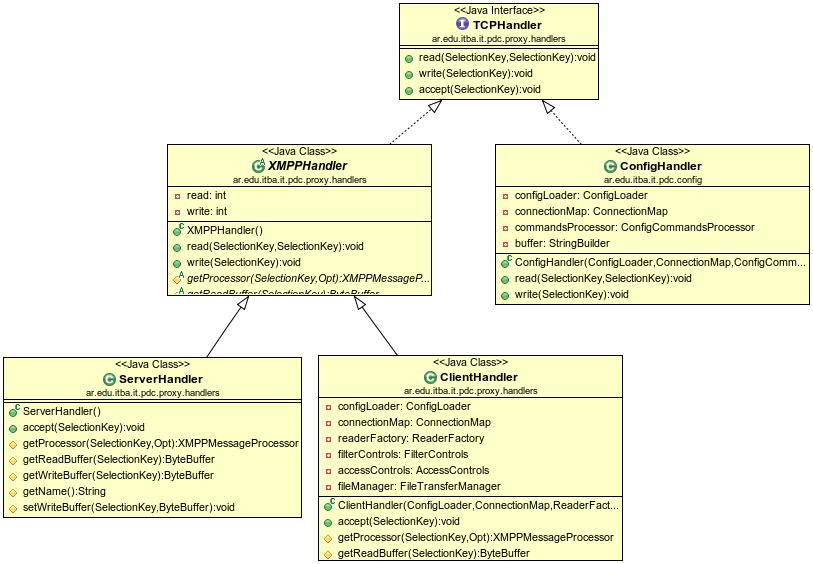
\includegraphics[width=400px]{UML/Handlers}  
	\caption{Diagrama UML de los handlers}
	\label{figure:Handlers}
\end{figure}

\newpage
\subsection{Elements}
\begin{figure}[h]
	\centering
	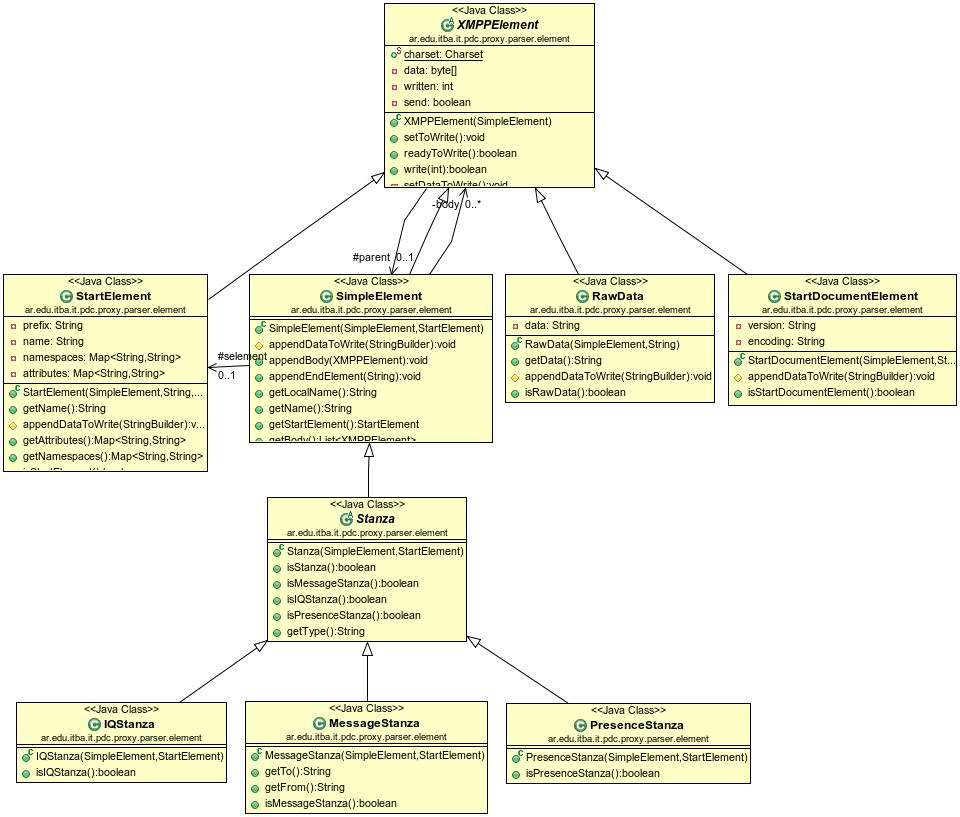
\includegraphics[width=400px]{UML/Elements}  
	\caption{Diagrama UML de los elementos XMPP}
	\label{figure:Elements}
\end{figure}

\newpage
\subsection{Processor}
\begin{figure}[h]
	\centering
	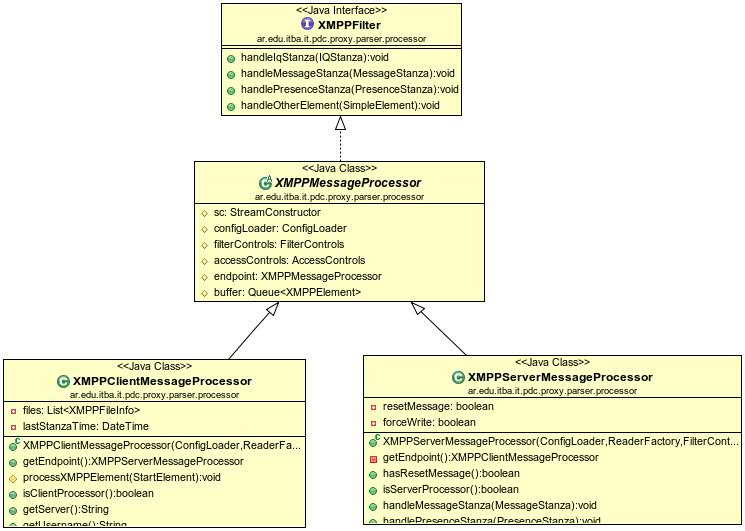
\includegraphics[width=400px]{UML/Processor}  
	\caption{Diagrama UML del mecanismo para procesar los streams}
	\label{figure:Processor}
\end{figure}

\newpage
\subsection{Configuración}
\begin{figure}[h]
	\centering
	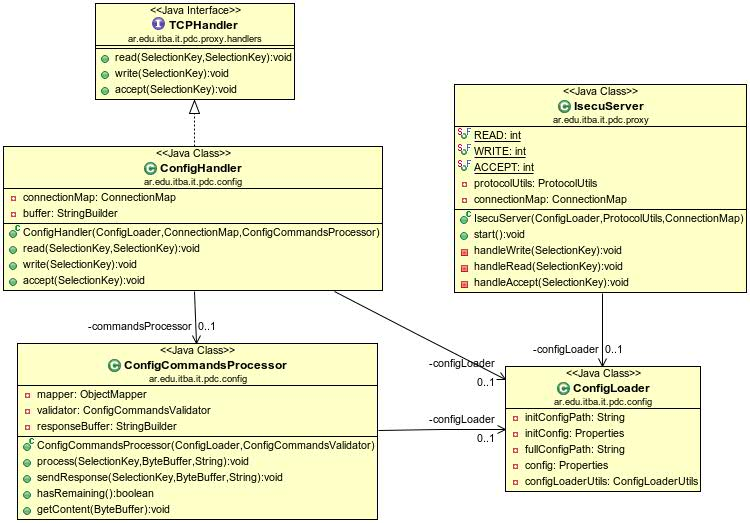
\includegraphics[width=400px]{UML/ConfigUML}  
	\caption{Diagrama UML del protocolo de configuración}
	\label{figure:ConfigUML}
\end{figure}

\end{document}
